\documentclass[12pt]{article}

\usepackage[utf8]{inputenc}
\usepackage[brazilian]{babel}
\usepackage{hyperref}
\usepackage{lipsum}
\usepackage{geometry}
\usepackage[skip=5pt plus1pt, indent=20pt]{parskip}
\usepackage{indentfirst}
\usepackage{amsthm,amssymb,amsmath}
\usepackage{minted}
\usepackage{graphicx}

\geometry{left=3cm, top=3cm, right=2cm, bottom=2cm}

\title{\textbf{Engenharia de Software 2 - Relatório TP1}}
\author{\textbf{Matheus Flávio Gonçalves Silva - 2020006850}}
\date{\parbox{\linewidth}{\centering%
		Universidade Federal de Minas Gerais (UFMG)\endgraf
		Belo Horizonte - MG - Brasil\endgraf\bigskip
		\href{mailto:matheusfgs@ufmg.br}{matheusfgs@ufmg.br}}}

\begin{document}
	
	\maketitle
	
	%%%%%%%%%%%%%%%%%%%%%%%%%%%%%%%%%%%%%%%%%%%%%%%%%%%%%%%%%%%%%%%%%%%%%%%%%%%%%%
	
	\section {Membros}
	Matheus Flávio Gonçalves Silva
	
	
	\section{Análise de qualidade com Lizard}
	\subsection{Execução da Ferramenta Lizard}
	\begin{figure}[h]
		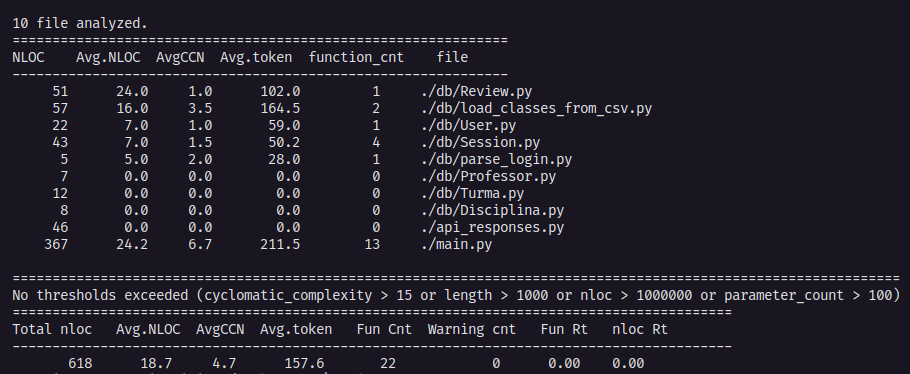
\includegraphics[scale=0.52]{Figure1.png}
		\caption{Saída da execução da ferramenta Lizard no Backend}	
	\end{figure}
	\par Conforme visto acima, a maioria das funciondalidades estão localizadas no arquivo \textbf{main.py}. Assim sendo, o foco da análise e modificação manter-se-á nas funções presentes nesse arquivo.
	
	\subsection{Análise da Função mais complexa}
	\par Ao analisar o código, a função mais complexa é a função \textbf{fetch\_review()}. Esta função está diretamente relacionada com a filtragem e ordenação das reviews de acordo com o semestre, professor, disciplina, classificação, podendo ser dinamicamente alterada de acordo com a preferência do usuário em tempo de uso.
	\par Assim sendo, essa função faz uso de consultas ao banco de dados com base nos filtros fornecidos, além de realizar o processamento dos resultados retornados pelo banco e retorna os dados obtidos como resposta ao frontend para exibição correta das reviews. Trata-se da função mais importante do sistema, afinal, de nada adianta fazer uma review a respeito de qualquer coisa que seja e essas reviews não serem exibidas.
	\par Dentre as estruturas e paradigmas envolvidos na função, temos a manipulação de listas, a utilização de filtros de pesquisa, além da ordenação dinâmica de acordo com a seleção do usuário.
	
	\section {Adicionais}
	\par A partir desse ponto, encontram-se explicações e documentações adicionais que não foram exigidas no PDF segundo o TP. Contudo, por questão de facilidade, foram acrescentadas a partir dessa sessão para maior conforto. Os items 1 e 3 pedidos na especificação encontram-se a seguir.
	
	\newpage
	
	\section {Explicação sobre o sistema}
	Para esse sistema web é idealizado um fórum de avaliação a respeito de professores da UFMG com dados referentes ao período de 2020/1 a 2023/1, seleção do semestre lecionado, além da validação se o professor deu aula da matéria especificada no semestre selecionado. Além disso, pode-se selecionar se serão feitas avaliações de forma anônima ou sem anonimato de acordo com a escolha do usuário ao criar a postagem.
	
	\section {Tecnologias}
	\begin {itemize}
	\item Quart (Backend)
	\par Foi escolhido o Quart como backend pela facilidade da manipulação da linguagem Python e pela similaridade com o framework Flask utilizado para desenvolvimento Web. De certo modo, pode-se dizer que o Quart é a reimplementação do Flask com a possibilidade de execução de funções assíncronas.
	\item React (Frontend)
	\par Foi escolhido o React como ferramenta para desenvolvimento do frontend pela maior intimidade com esse framework.
	\item MongoDB (Banco de Dados)
	\par Para o banco de dados foi escolhido o MongoDB pela possibilidade de utilização do MongoDB Compass facilitar a correção de pequenos problemas, a visualização dos dados e correção do banco. Foram cogitados também os bandos MySQL e SQLite, mas deixados de lado em virtude da experiência de maior facilidade de lidar com o MongoDB. 
	\end {itemize}
	
	\section{Refatoração}
	
	\par \href{https://github.com/matheusflavio/ES2-TP-uni-opinions/commit/513604ddffb299875afa250f774080f2add1972a}{Refactoring 1}
	\par \href{https://github.com/matheusflavio/ES2-TP-uni-opinions/commit/513604ddffb299875afa250f774080f2add1972a}{Refactoring 2}
\end{document}
